\section{Dropbox}
\subsection{Giới thiệu về Dropbox}
Dropbox là một ứng dụng lưu trữ và chia sẽ dữ liệu trực tuyến. Bất cứ tài liệu nào lưu vào Dropbox cũng đều được đồng bộ lên web và các thiết bị khác có kết nối đến Dropbox của bạn hoặc những người được chia sẽ mới có thể truy cập vào dữ liệu của bạn.
\begin{list}{--}{}
\item Ưu điểm: tốc độ tải nhanh, có khả năng đồng bộ hóa dữ liệu trên web và máy tính (hoặc thiết bị di động) khi có kết nối internet.
\item Nhược điểm: Dung lượng miễn phí chỉ được $2GB$ lưu trữ.
\item Cách tăng dung lượng sử dụng miễn phí: với mỗi người được bạn mời sử dụng Dropbox (thông qua liên kết của bạn) thì được tăng thêm $500MB$ trên một lượt, dung lượng miễn phí tối đa là $16GB$.
\end{list}
\subsection{Đăng ký tài khoản Dropbox}\label{Sub:sign-up-dropbox}
Truy cập vào địa chỉ \texttt{https://www.dropbox.com/} để đăng ký tải khoản Dropbox (nếu bạn chưa có tài khoản).
\begin{figure}[!h]
\begin{center}
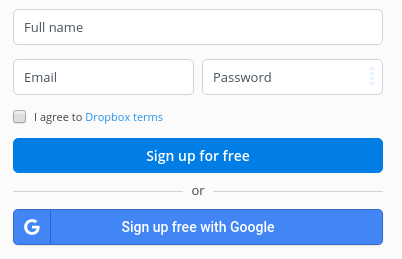
\includegraphics[scale=.7]{images/sign-up-dropbox.png} 
\end{center}
\caption{Đăng ký tài khoản Dropbox}\label{Fig:Sign-up-Dropbox}
\end{figure}

Nếu bạn chưa có tài khoản \verb|Gmail| thì làm theo hướng dẫn bên dưới:
\begin{list}{--}{}
\item Điền thông tin tài khoản Dropbox sau này:
\begin{list}{+}{}
\item Ô \verb|Full name|: điền tên bạn muốn hiển thị.
\item Ô \verb|Email|: điền Email của bạn.
\item Ô \verb|password|: nhập mật khẩu đăng nhập sau này vào đây.
\item[$\ast$] Đây cũng là địa chỉ và mật khẩu bạn đăng nhập vào Dropbox sau này. Cần ghi nhớ \verb|Email| và \verb|Password|.
\end{list}
\item Click chọn \verb|I agree to Dropbox terms|.
\item Click chọn \verb|Sign up for free|.
\end{list}
Nếu bạn đã có tài khoản \verb|Gmail| thì dùng tài khoản \verb|Gmail| để đăng ký \verb|Dropbox|, click chọn \verb|Sign up free with Google| (hình \ref{Fig:Sign-up-Dropbox}).
\begin{list}{--}{}
\item Có thể bạn sẽ cần nhập lại địa chỉ \verb|Gmail| và \verb|Password| của địa chỉ \verb|Gmail| để đăng nhập \verb|Gmail| xác nhận thông tin.
\item Thông tin cần xác nhận như hình \ref{Fig:Sign-up-Dropbox-by-Gmail}: chọn \verb|Allow| để xác nhận.
\begin{figure}[!h]
\begin{center}
\subfloat[Chọn \textsf{Allow}\label{Fig:Sign-up-Dropbox-by-Gmail}]
	{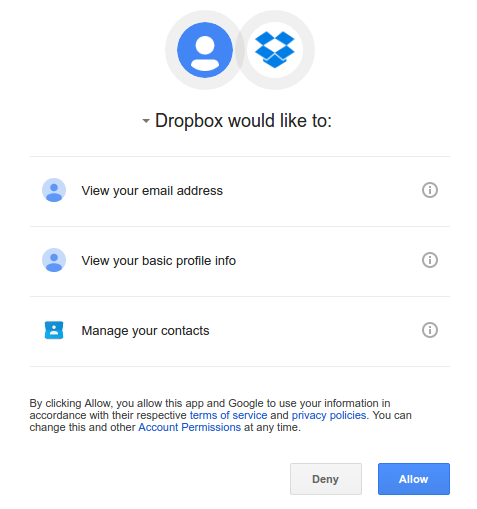
\includegraphics[scale=.5]{images/signup-dropbox-by-gmail.png}} \hspace{.5cm}
\subfloat[Điền thông tin tài khoản\label{Fig:account-Dropbox-by-Gmail}]
	{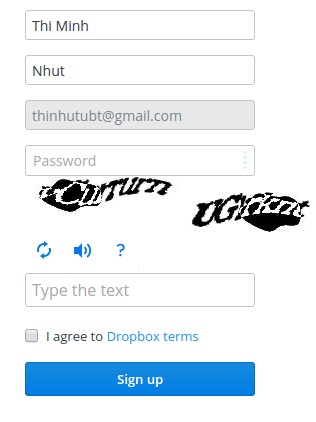
\includegraphics[scale=.5]{images/creat-account-dropbox-by-gmail.png}}
\end{center}
\caption{Sử dụng địa chỉ \textsl{Gmail} để đăng ký \textsf{Dropbox}}
\end{figure}
\item Điền thông tin cho tài khoản Dropbox sau này, thông tin trong hình \ref{Fig:account-Dropbox-by-Gmail}:
\begin{list}{+}{}
\item Ô \verb|Password|: Nhập vào mật khẩu đăng nhập Dropbox sau này.
\item Ô \verb|Type the text|: Nhập vào mã xác nhận.
\item Click chọn \verb|I agree to Dropbox terms|.
\item Click chọn \verb|Sign up|.
\end{list}
\end{list}
\subsection{Cài đặt Dropbox}
Vào \verb|Ubuntu Software Center|, tìm ứng dụng \verb|Dropbox| (như hình \ref{Fig:Install-Dropbox}), click chọn \verb|Install| để cài đặt ứng dụng cho máy tính.
\begin{figure}[!h]
\begin{center}
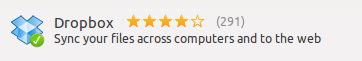
\includegraphics[scale=.7]{images/Install-Dropbox.png} 
\end{center}
\caption{Ứng dụng \textsf{Dropbox} trong \textsf{Ubuntu Software Center}}\label{Fig:Install-Dropbox}
\end{figure}
\subsection{Sử dụng Dropbox đồng bộ dữ liệu giữa máy tính và dữ liệu trên web}
\begin{list}{--}{}
\item Mở ứng dụng \verb|Dopbox| vừa cài đặt (tìm trong thanh \verb|Dash|) như hình \ref{Fig:app-dropbox}:
\begin{figure}[!h]
\begin{center}
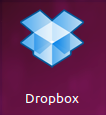
\includegraphics[scale=.5]{images/app-dropbox.png} 
\end{center}
\caption{Ứng dụng \textsf{Dropbox} trên \textsf{Ubuntu}} \label{Fig:app-dropbox}
\end{figure}
\item Điền địa chỉ \verb|Email| và \verb|Password| đã đăng ký ở mục \ref{Sub:sign-up-dropbox}: hình 
\begin{figure}[!h]
\begin{center}
\subfloat[Điền thông tin đăng nhập \textsf{Dropbox} \label{Fig:account-dropbox}]
	{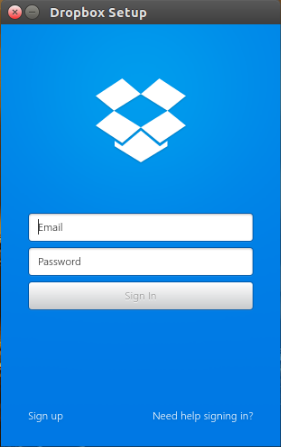
\includegraphics[scale=.4]{images/sync-dropbox.png}} \hspace{.5cm}
	\subfloat[Chọn \textsf{Open my Dropbox folder} \label{Fig:open-dropbox-folder}]
	{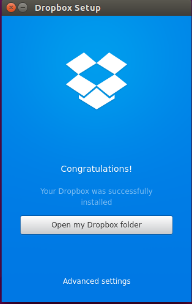
\includegraphics[scale=.58]{images/sync-dropbox-folder.png}} \hspace{.5cm}
\end{center}
\caption{Mở ứng dụng \textsf{Dropbox} trên \textsf{Ubuntu}}
\end{figure}
\end{list}
\subsection{Các lệnh của ứng dụng Dropbox}
\begin{list}{--}{}
\item[]Các lệnh dùng để tương tác với \verb|Dropbox|
\begin{lstlisting}[language=bash]
Dropbox command-line interface

commands:

Note: use dropbox help <command> to view usage for a specific command.

 status       get current status of the dropboxd
 help         provide help
 puburl       get public url of a file in your dropbox
 stop         stop dropboxd
 running      return whether dropbox is running
 update       download latest version of dropbox
 start        start dropboxd
 filestatus   get current sync status of one or more files
 ls           list directory contents with current sync status
 autostart    automatically start dropbox at login
 exclude      ignores/excludes a directory from syncing
 lansync      enables or disables LAN sync
\end{lstlisting}
\end{list}